\documentclass{article}
\usepackage[utf8]{inputenc}
\usepackage{graphicx}
\usepackage[dvipsnames]{xcolor}
\usepackage{listings}
\usepackage{float}
\usepackage{pdfpages}

\newcommand\YAMLcolonstyle{\color{red}\mdseries}
\newcommand\YAMLkeystyle{\color{black}\bfseries}
\newcommand\YAMLvaluestyle{\color{blue}\mdseries}

\makeatletter

% here is a macro expanding to the name of the language
% (handy if you decide to change it further down the road)
\newcommand\language@yaml{yaml}

\expandafter\expandafter\expandafter\lstdefinelanguage
\expandafter{\language@yaml}
{
  keywords={true,false,null,y,n},
  keywordstyle=\color{darkgray}\bfseries,
  basicstyle=\YAMLkeystyle,                                 % assuming a key comes first
  sensitive=false,
  comment=[l]{\#},
  morecomment=[s]{/*}{*/},
  commentstyle=\color{purple}\ttfamily,
  stringstyle=\YAMLvaluestyle\ttfamily,
  moredelim=[l][\color{orange}]{\&},
  moredelim=[l][\color{magenta}]{*},
  moredelim=**[il][\YAMLcolonstyle{:}\YAMLvaluestyle]{:},   % switch to value style at :
  morestring=[b]',
  morestring=[b]",
  literate =    {---}{{\ProcessThreeDashes}}3
                {>}{{\textcolor{red}\textgreater}}1     
                {|}{{\textcolor{red}\textbar}}1 
                {\ -\ }{{\mdseries\ -\ }}3,
}

% switch to key style at EOL
\lst@AddToHook{EveryLine}{\ifx\lst@language\language@yaml\YAMLkeystyle\fi}
\makeatother

\newcommand\ProcessThreeDashes{\llap{\color{cyan}\mdseries-{-}-}}


\newcommand{\namedlisting}[2][]{%
    \lstinputlisting[caption={\texttt{\detokenize{#2}}},#1]{#2}%
}

\newcommand*\lstinputpath[1]{\lstset{inputpath=#1}}

% "define" Scala
\lstdefinelanguage{scala}{
  morekeywords={abstract,case,catch,class,def,%
    do,else,extends,false,final,finally,%
    for,if,implicit,import,match,mixin,%
    new,null,object,override,package,%
    private,protected,requires,return,sealed,%
    super,this,throw,trait,true,try,%
    type,val,var,while,with,yield},
  otherkeywords={=>,<-,<\%,<:,>:,\#,@},
  sensitive=true,
  morecomment=[l]{//},
  morecomment=[n]{/*}{*/},
  morestring=[b]",
  morestring=[b]',
  morestring=[b]"""
}

\usepackage{color}
\definecolor{dkgreen}{rgb}{0,0.6,0}
\definecolor{gray}{rgb}{0.5,0.5,0.5}
\definecolor{mauve}{rgb}{0.58,0,0.82}

\lstset{frame=tb,
  language=scala,
  aboveskip=3mm,
  belowskip=3mm,
  showstringspaces=false,
  columns=flexible,
  basicstyle={\small\ttfamily},
  numbers=none,
  numberstyle=\tiny\color{gray},
  keywordstyle=\color{blue},
  commentstyle=\color{dkgreen},
  stringstyle=\color{mauve},
  breaklines=true,
  breakatwhitespace=true
  tabsize=1
}

\title{FullCart WebShop}
\author{Katona, Áron}
\date{\parbox{\linewidth}{\centering%
  Team\endgraf\medskip
  Fodor, Zsófia \hspace*{3cm} Katona, Áron\endgraf\bigskip
  \today\endgraf
  }}


\begin{document}
\pagenumbering{gobble}
\maketitle

\newpage
\pagenumbering{roman}

\begin{abstract}

The project is a proof-of-concept application for using session types for communication between micro-services in a distributed back-end. 

The application implements a webshop. It provides services for creating, viewing and managing user accounts, products and orders.

Another important factor is the list of technologies we used, and their purpose:

\begin{enumerate}
    \item Scala
    \item Spring Boot: webserver, database access (JPA)
    \item Maven: project, modules
    \item Docker: Containers for the services and for the databases
    \item Docker Compose: setting up all the containers at once
    \item Scribble, Scribble-Java \cite{HY2016}: Session type generation
    \item REST+HATEOAS: communication protocl with the end-user
\end{enumerate}

The project is divided into modules, one for each micro-service. The back-end is split into 3 microservices:

\begin{itemize}
    \item Webshop(proxy) service: receives HTTP requests and responds to them
    \item Product service: manages the products
    \item User service: manages the users
    \item Buying service: manages the orders placed by the user
\end{itemize}

The proxy provides the REST endpoints and calls the other micro-services via the session types, in order to fulfill the requests.


My responsibility was the implementation of the:

\begin{itemize}
    \item Buying Service
    \item Webshop Service
    \item BuyingSession protocol
    \item Maven project configuration
    \item Containerization
\end{itemize}

\end{abstract}

\newpage
\tableofcontents

\newpage
\pagenumbering{arabic}



% \chapter{Mini Project}
% 
% \lstinputpath{../webshop-single/src/main/java/com/fullcart/webshop/}
% 
% \namedlisting[]{model/OrderStatus.java}
% 
% \lstinputpath{../webshop-single/src/main/scala/com/fullcart/webshop/}
% 
% \namedlisting[]{controller/ProductController.scala}
% \namedlisting[]{controller/UserController.scala}
% \namedlisting[]{controller/RootController.scala}
% \namedlisting[]{controller/OrderController.scala}
% 
% \namedlisting[]{transformer/OrderDTOTransformer.scala}
% 
% \namedlisting[]{dto/OrderDTO.scala}
% 
% \namedlisting[]{WebshopApplication.scala}
% 
% 
% \namedlisting[]{model/assembler/UserModelAssembler.scala}
% \namedlisting[]{model/assembler/OrderModelAssembler.scala}
% \namedlisting[]{model/assembler/ProductModelAssembler.scala}
% \namedlisting[]{model/Order.scala}
% \namedlisting[]{model/User.scala}
% \namedlisting[]{model/Product.scala}
% 
% \namedlisting[]{repository/OrderRepository.scala}
% \namedlisting[]{repository/ProductRepository.scala}
% \namedlisting[]{repository/UserRepository.scala}
% 
% \namedlisting[]{uriconverter/UserUriConverter.scala}
% \namedlisting[]{uriconverter/AbstractUriConverter.scala}
% \namedlisting[]{uriconverter/ProductUriConverter.scala}
% \namedlisting[]{uriconverter/UriConverter.scala}
% 
% \subsubsection{Resources}
% \lstinputpath{../webshop-single/src/main}
% \namedlisting[]{resources/application.yml}
% 
% 
% \subsection{Pom file}
% \lstinputpath{../webshop-single/}
% \namedlisting[]{pom.xml}
% 
% \chapter {Final Project}

\section{Design}

\subsection{Use Case Diagram}
  
\begin{figure}[H]
    \centering
    \includegraphics[width=\linewidth]{img/usecases.png}
    \caption{Use Case diagram}
\end{figure}
    
\subsection {Models}
    
\begin{figure}[H]
    \centering
    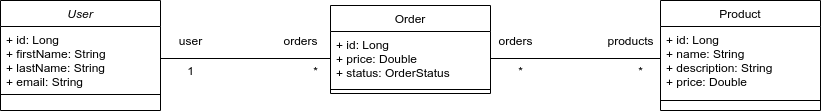
\includegraphics[width=\linewidth]{img/Models.png}
    \caption{Models of the application}
\end{figure}


\subsection{Protocols}

\subsubsection{Protocol specification}

\lstinputpath{../webshop-distributed/common/src/main/scribble/}

Listing \ref{lst:protocol} contains the protocol specification in the Scribble language. The following protocols were defined:

\begin{itemize}
    \item \textbf{ProductSession:} protocol for communication with the product service
    
    \item \textbf{UserSession:} protocol for communication with the user service
    
    \item \textbf{BuyingSession:} protocol for communication with the buying service, which also communicates with the User and Product service.
\end{itemize}

\namedlisting[label={lst:protocol}]{Webshop.scr}

\subsubsection{Endpoint finite-state-machines from the client's point of view}

[Next 3 pages]

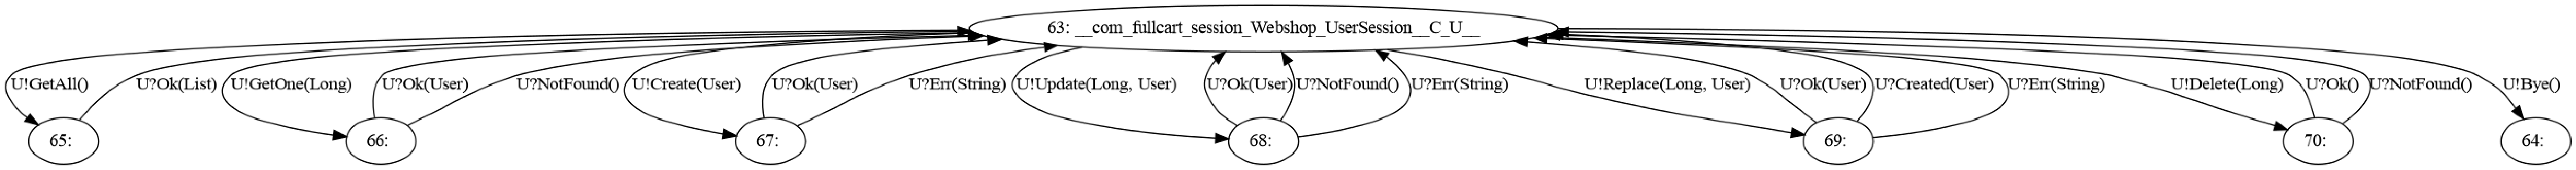
\includepdf[pages=-,fitpaper]{img/protocols/UserSession_C.pdf}
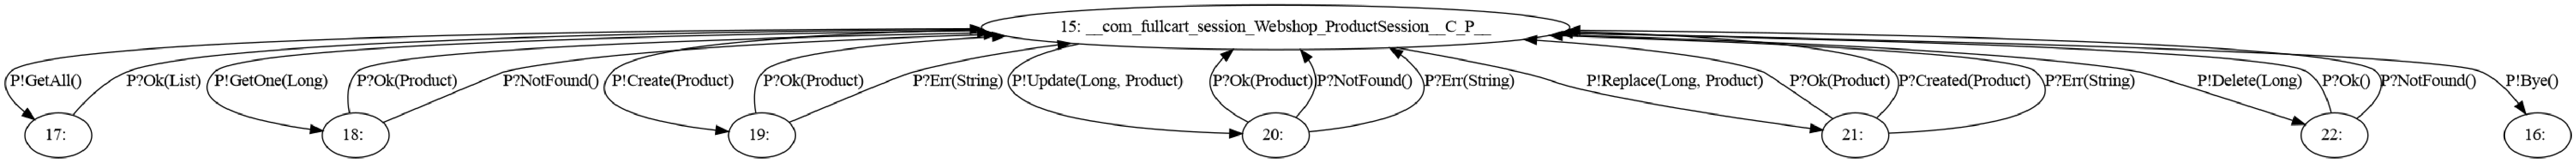
\includepdf[pages=-,fitpaper]{img/protocols/ProductSession_C.pdf}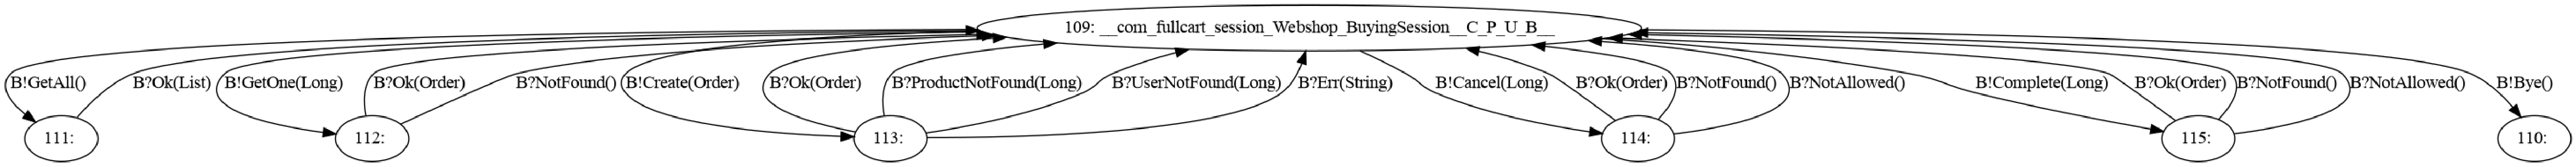
\includepdf[pages=-,fitpaper]{img/protocols/BuyingSession_C.pdf}
    
\subsection {Services}
  
\begin{figure}[H]
    \centering
    \includegraphics[width=\linewidth]{img/services.png}
    \caption{Overview of the micro-services}
\end{figure}

\subsection {Deployment}
  
The application is deployed in Docker containers. Each container represents an independent server computer. 

For each micro-service a separate docker container was created. For those services that need a database, a separate MySQL container was associated. These databases are accessible to the service through the specified port, but inaccessible to any other containers.

The services communicate with each other through a specified port, using the protocols defined in the session types.

\subsubsection{Deployment Diagram}
\begin{figure}[H]
    \centering
    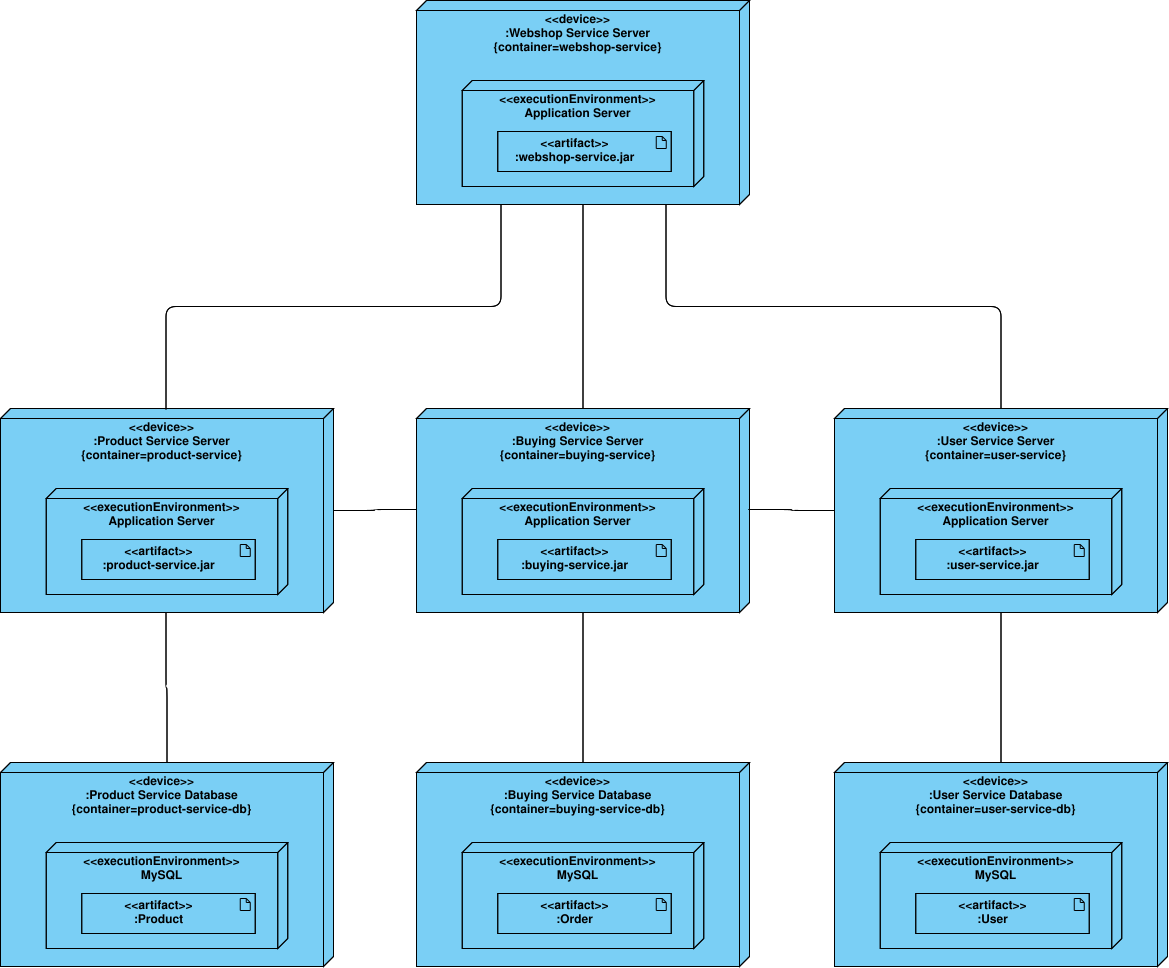
\includegraphics[width=\linewidth]{img/Deployment.png}
    \caption{Overview of the micro-services}
\end{figure}


% \subsection {Class diagrams}
% 
% The following pages contain the generated class diagrams for each service. Because of the dependency injection, provided by the Spring framework, the UML generator tool did not show the dependencies between the classes. Morevoer because the Scala language was used, the UML diagrams show methods instead of fields.
% 
% 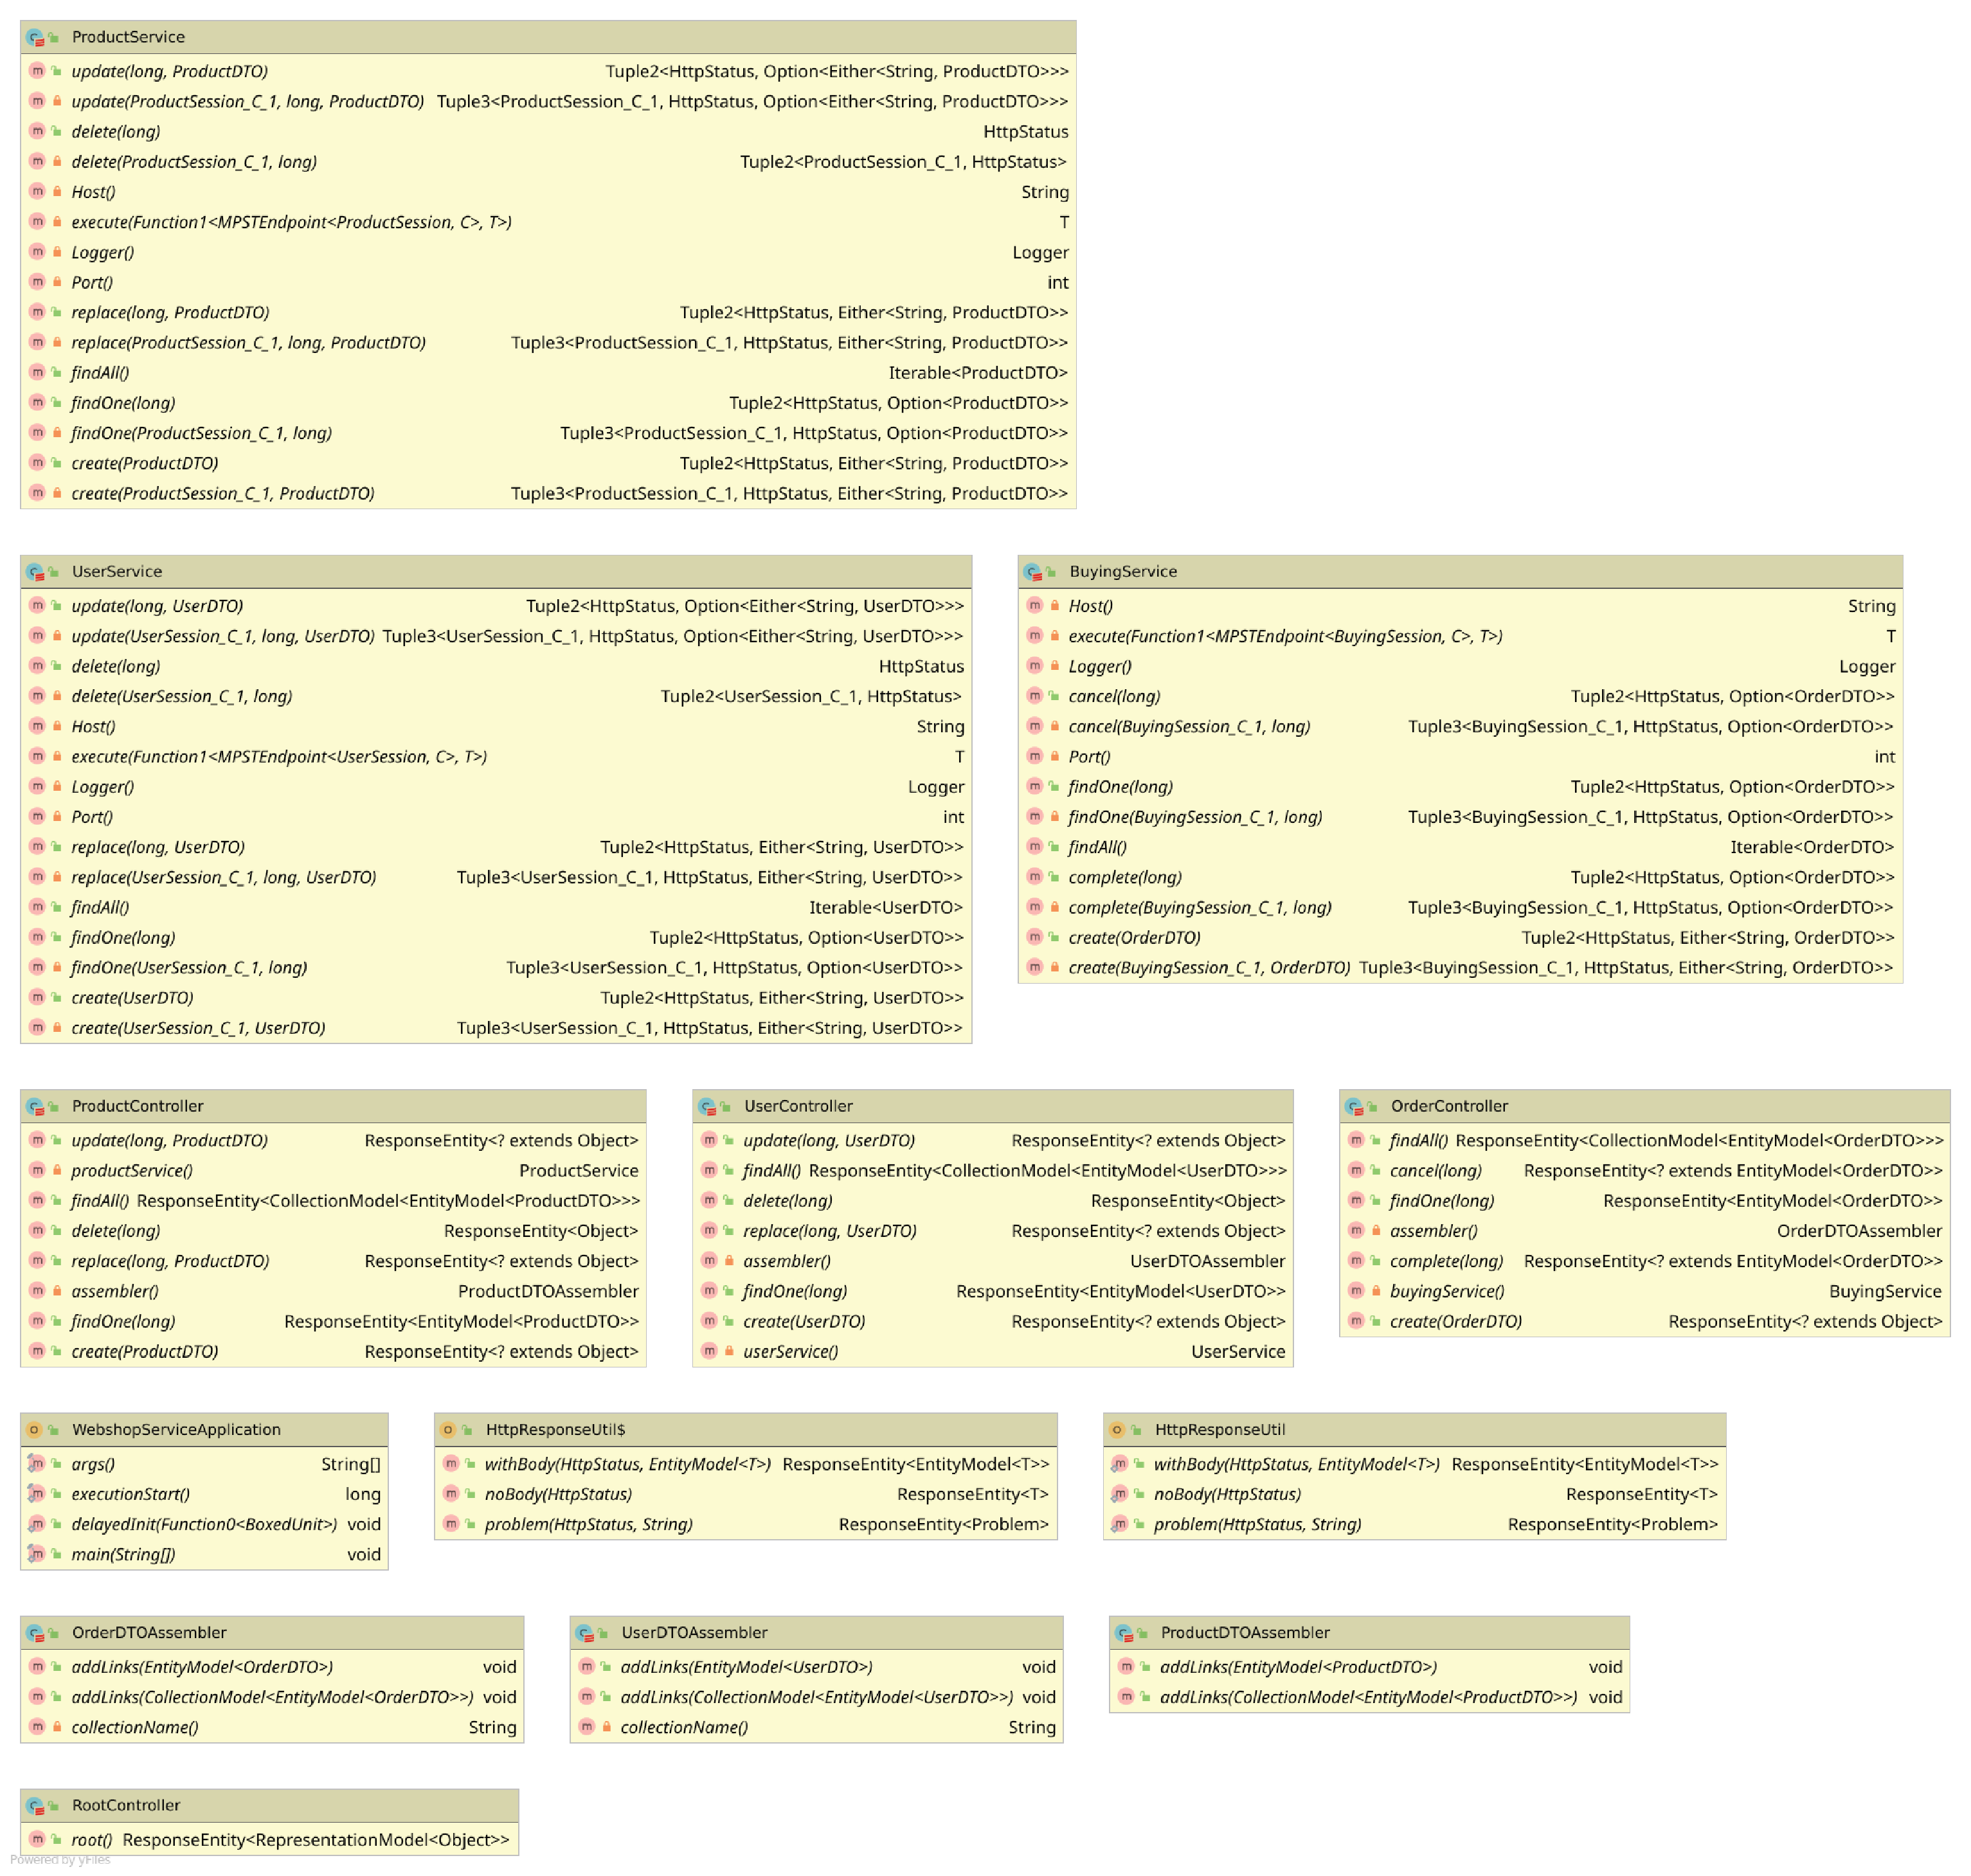
\includepdf[pages=-,fitpaper]{img/class-webshop.pdf}
% 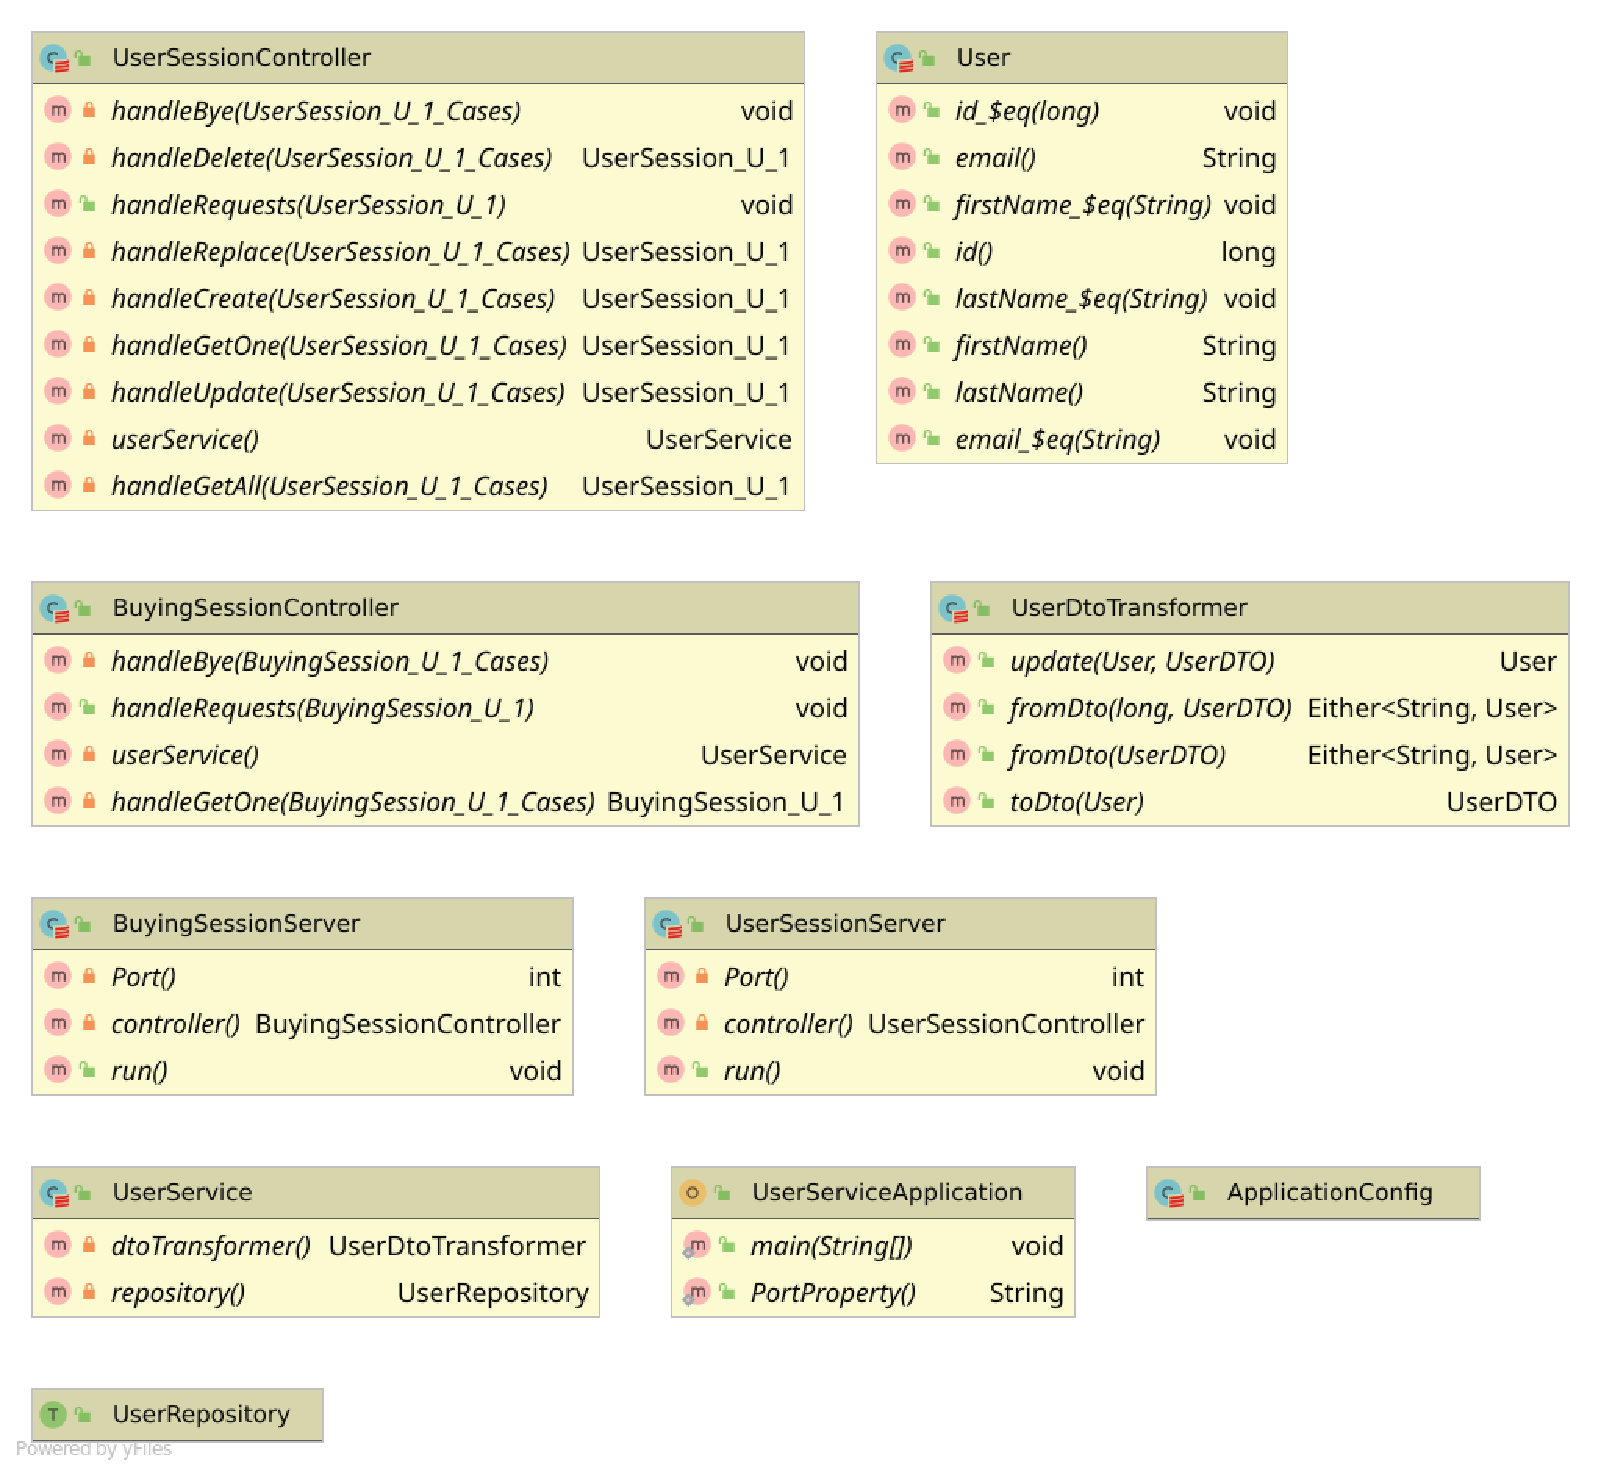
\includepdf[pages=-,fitpaper]{img/class-user.pdf}
% 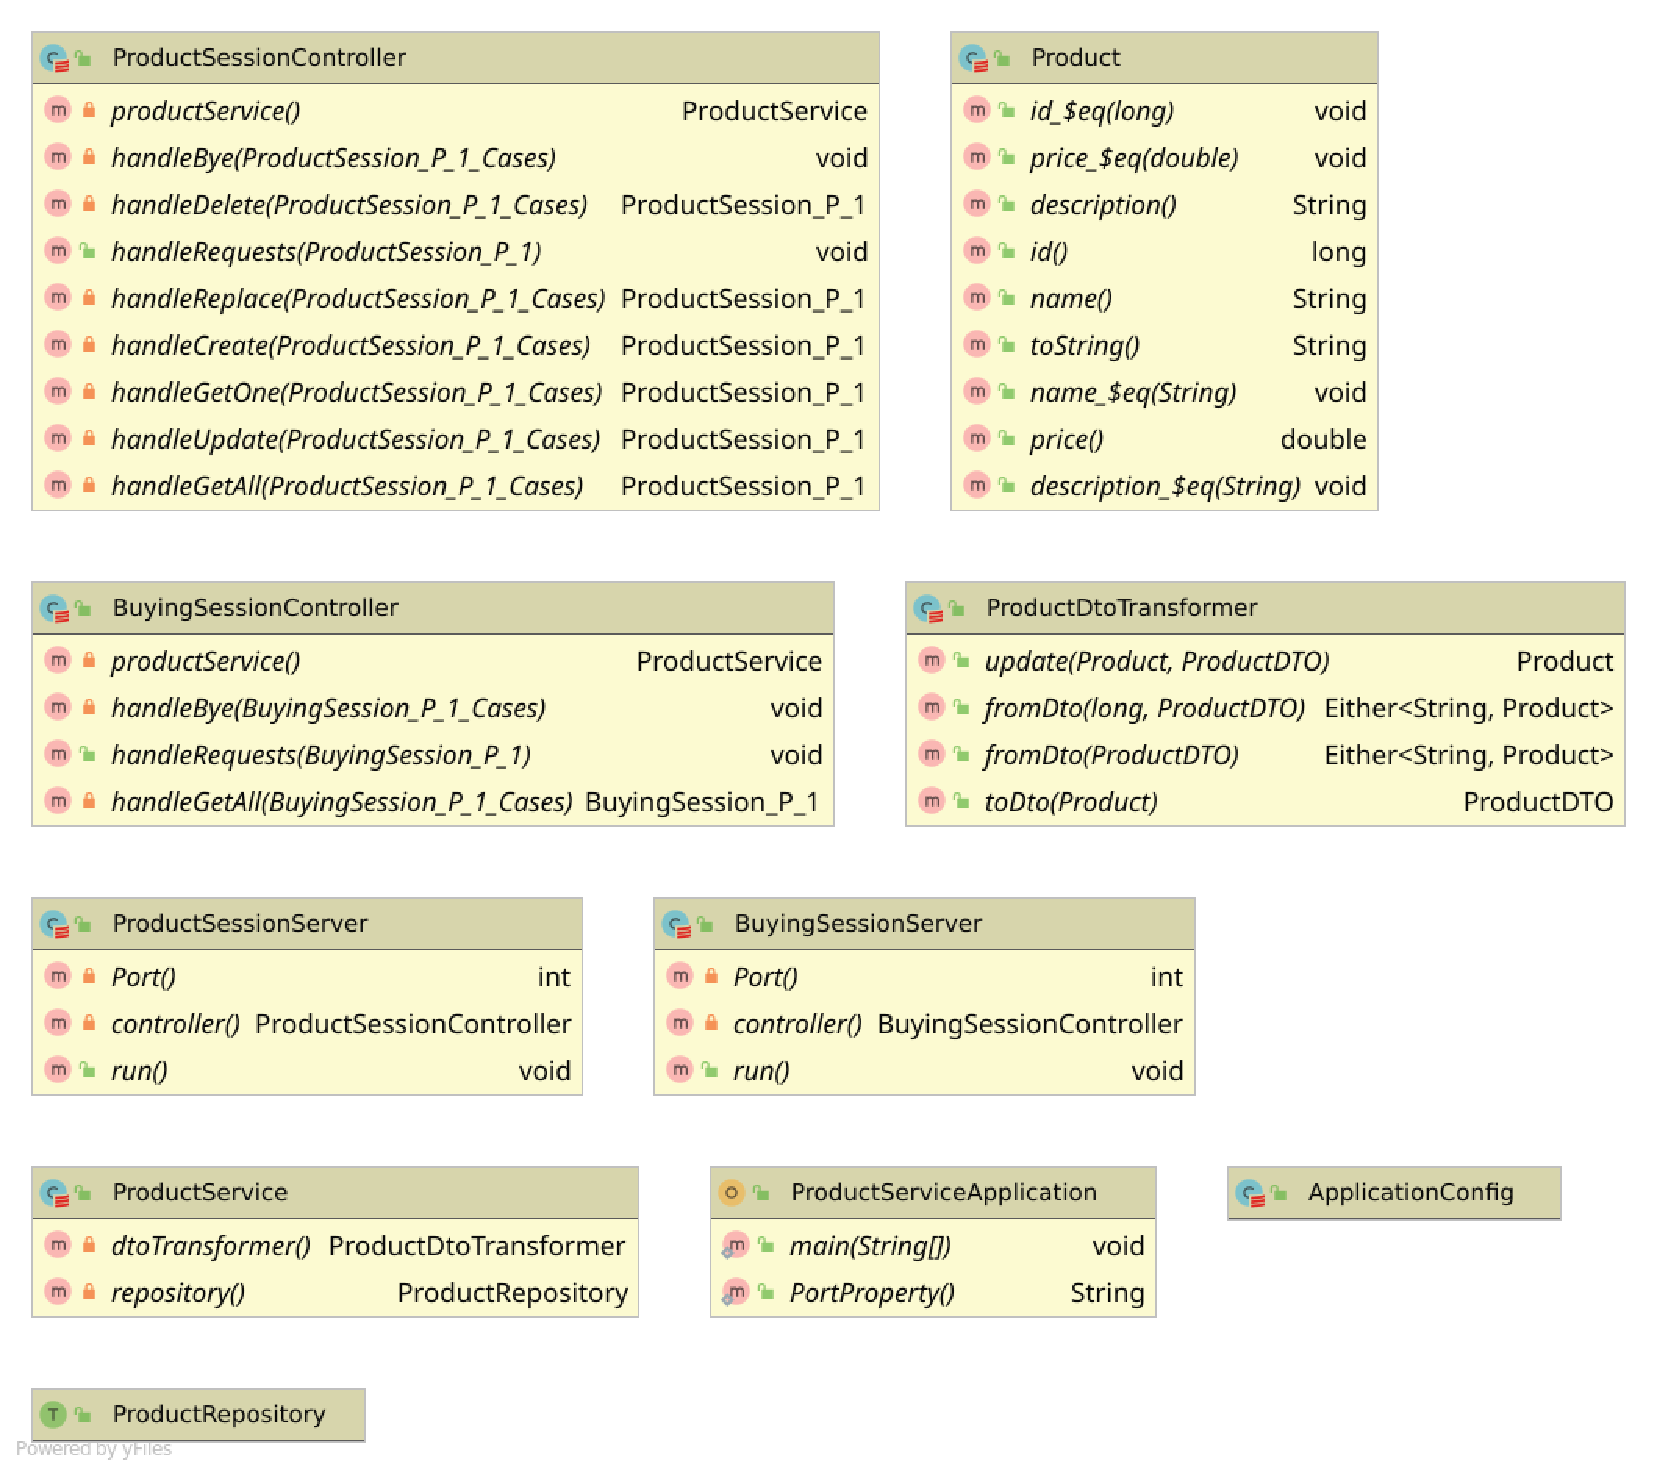
\includepdf[pages=-,fitpaper]{img/class-product.pdf}
% 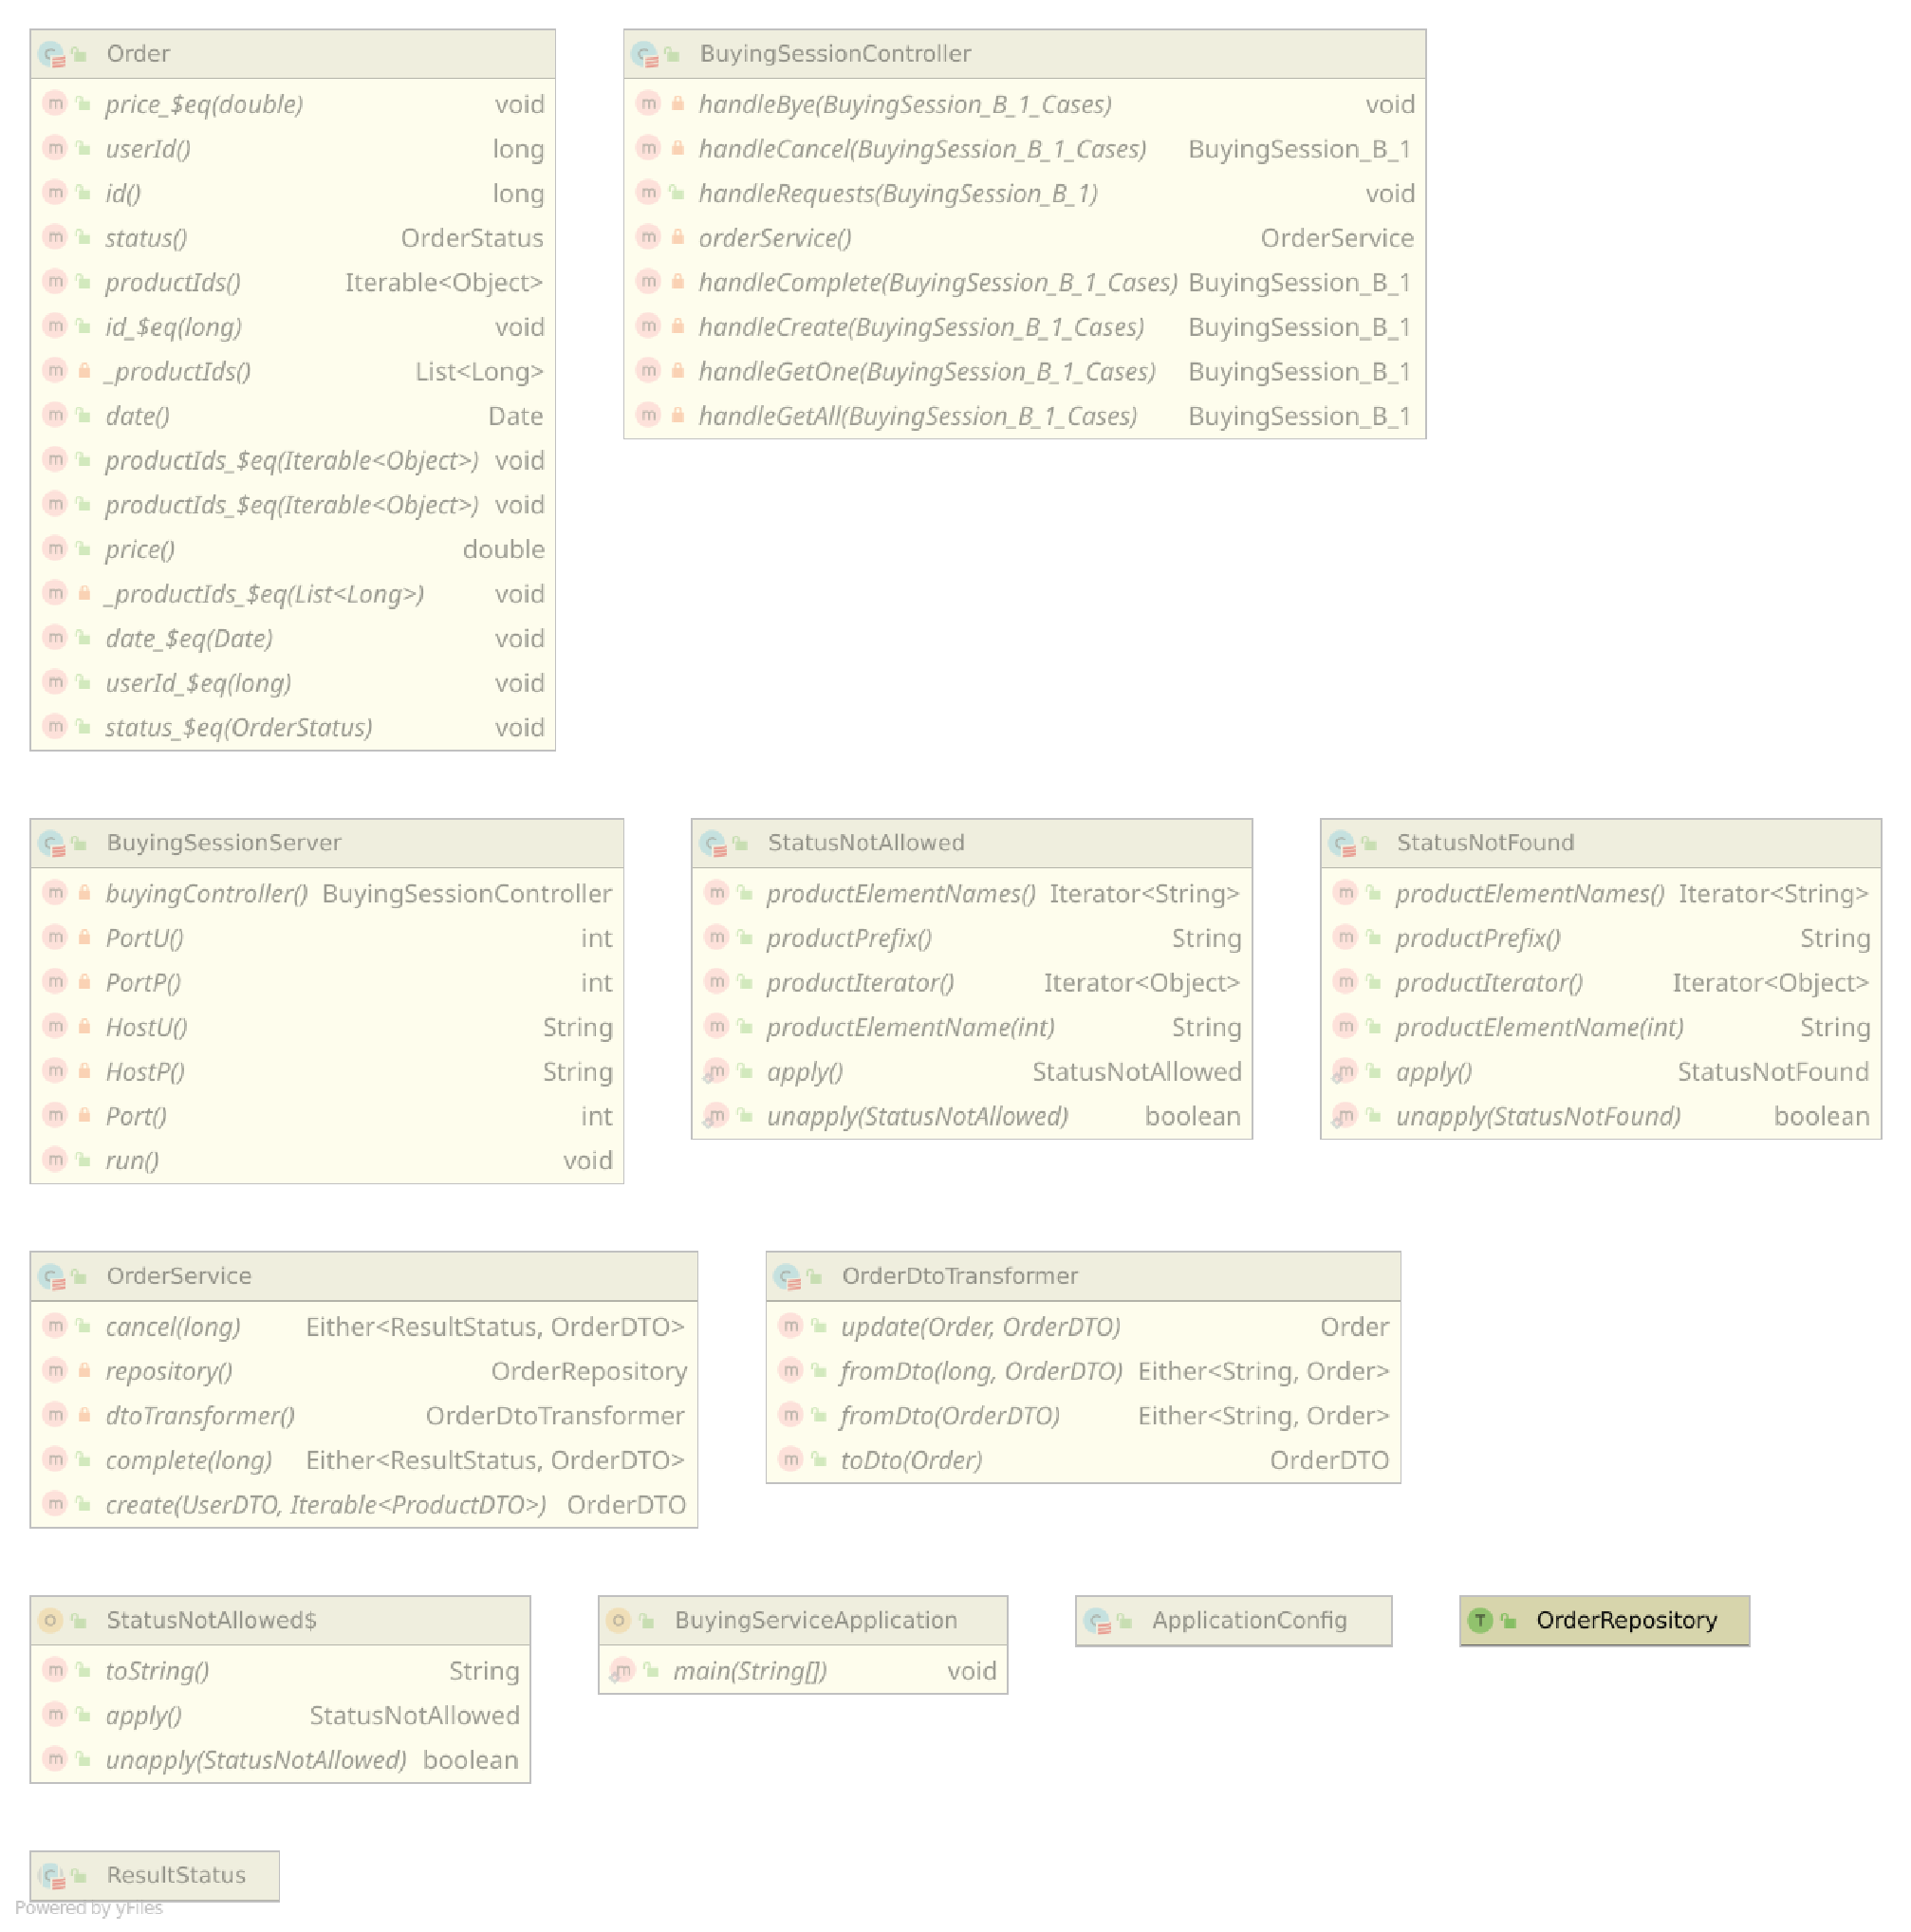
\includepdf[pages=-,fitpaper]{img/class-buying.pdf}
% 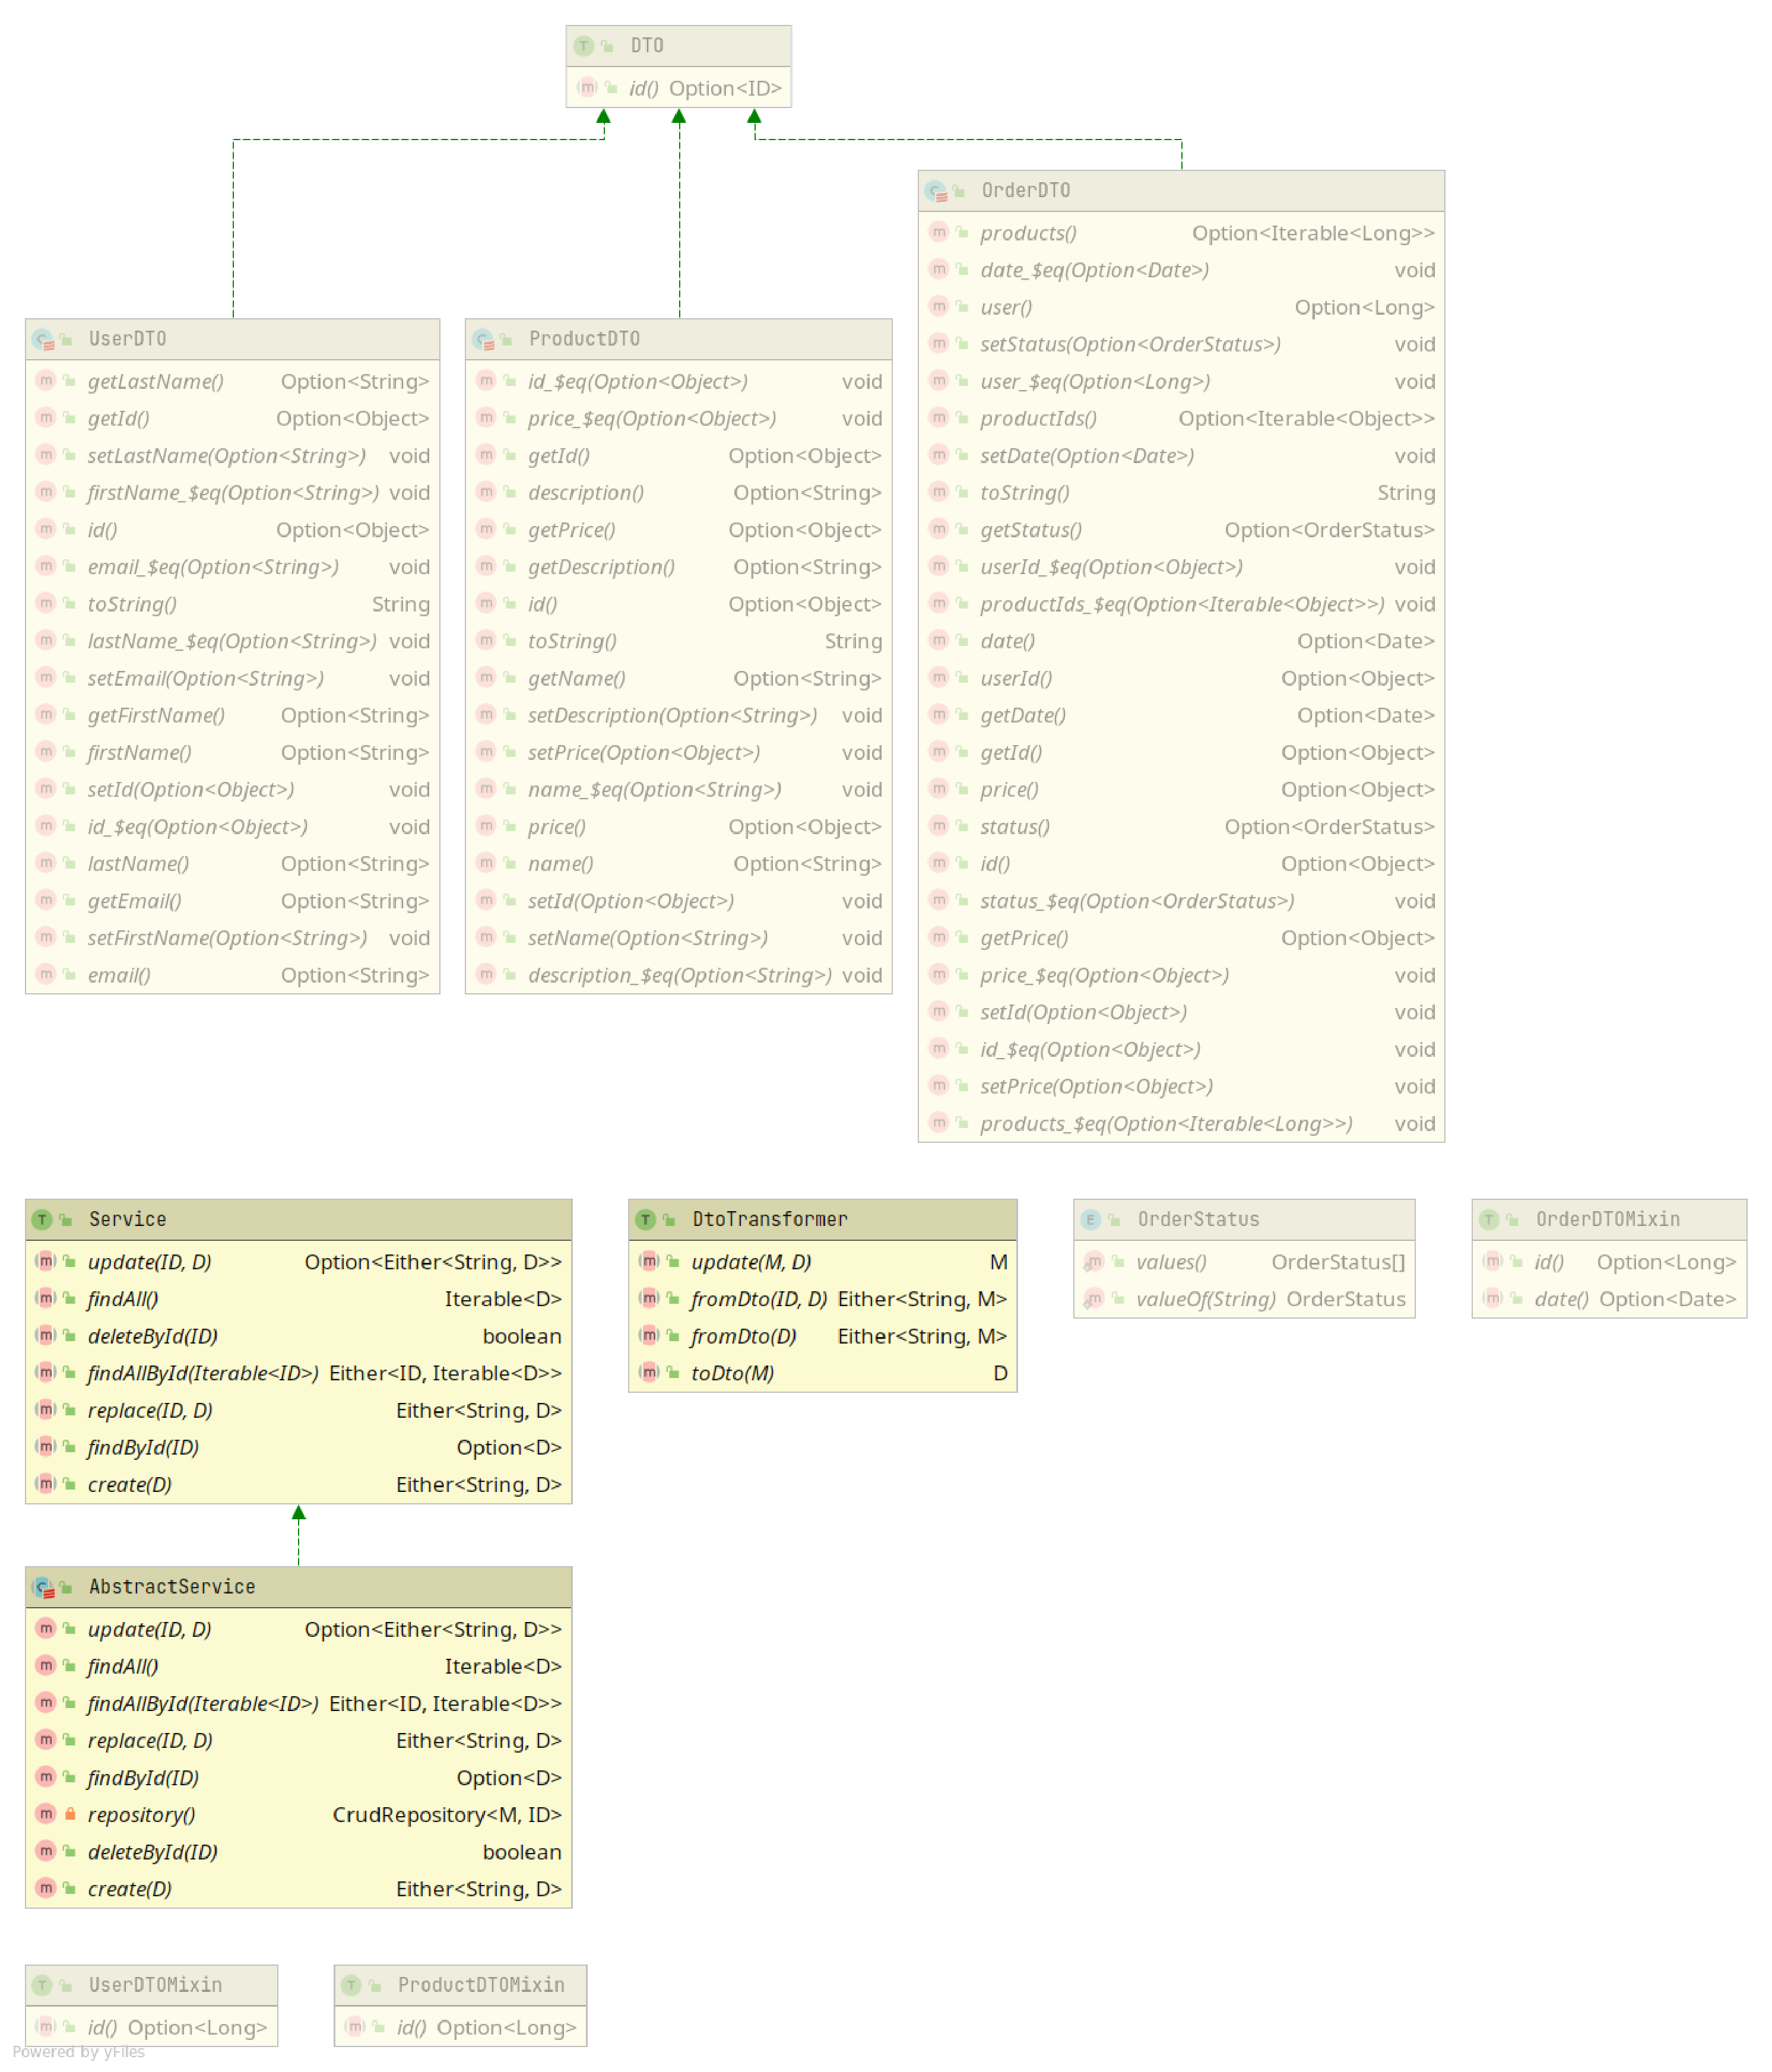
\includepdf[pages=-,fitpaper]{img/class-common.pdf}



% \section{Source Code}
% 
% \subsection{Docker compose file}
% \lstinputpath{../webshop-distributed/}
% \namedlisting[language=yaml]{docker-compose.yml}
% 
\subsection{Sample .env file}
This file must be placed next to `the docker-compose.yml` file.

\lstinputpath{../webshop-distributed/sample.env/}
\namedlisting[]{.env}
% \subsection{Webhsop-service}
% \lstinputpath{../webshop-distributed/webshop-service/src/main/scala/com/fullcart/webshop/}
% 
% \namedlisting[]{WebshopServiceApplication.scala}
% \namedlisting[]{service/BuyingService.scala}
% 
% \namedlisting[]{controller/ProductController.scala}
% \namedlisting[]{controller/UserController.scala}
% \namedlisting[]{controller/OrderController.scala}
% \namedlisting[]{controller/RootController.scala}
% 
% \namedlisting[]{assembler/ProductDTOAssembler.scala}
% \namedlisting[]{assembler/OrderDTOAssembler.scala}
% \namedlisting[]{assembler/UserDTOAssembler.scala}
% 
% \namedlisting[]{util/HttpResponseUtil.scala}
% 
% \namedlisting[]{service/BuyingService.scala}
% \namedlisting[]{service/ProductService.scala}
% \namedlisting[]{service/UserService.scala}
% 
% \subsubsection{resources}
% \lstinputpath{../webshop-distributed/webshop-service/src/main/resources}
% 
% \namedlisting[]{application.yml}
% 
% \subsubsection{pom file}
% \lstinputpath{../webshop-distributed/webshop-service/}
% 
% \namedlisting[]{pom.xml}
% 
% \subsection{User-service}
% \lstinputpath{../webshop-distributed/user-service/src/main/scala/com/fullcart/user/}
% 
% \namedlisting[]{UserServiceApplication.scala}
% 
% \namedlisting[]{controller/BuyingSessionController.scala}
% \namedlisting[]{controller/UserSessionController.scala}
% 
% \namedlisting[]{service/UserDtoTransformer.scala}
% \namedlisting[]{service/UserService.scala}
% 
% \namedlisting[]{repository/UserRepository.scala}
% 
% \namedlisting[]{model/User.scala}
% 
% \namedlisting[]{server/UserSessionServer.scala}
% \namedlisting[]{server/BuyingSessionServer.scala}
% 
% \subsubsection{resources}
% \lstinputpath{../webshop-distributed/user-service/src/main/resources}
% 
% \namedlisting[]{application.yml}
% 
% \subsubsection{pom file}
% \lstinputpath{../webshop-distributed/user-service/}
% 
% \namedlisting[]{pom.xml}
% 
% \subsection{Product-service}
% \lstinputpath{../webshop-distributed/product-service/src/main/scala/com/fullcart/product/}
% 
% \namedlisting[]{controller/BuyingSessionController.scala}
% \namedlisting[]{controller/ProductSessionController.scala}
% 
% \namedlisting[]{service/ProductDtoTransformer.scala}
% \namedlisting[]{service/ProductService.scala}
% 
% \namedlisting[]{repository/ProductRepository.scala}
% 
% \namedlisting[]{model/Product.scala}
% 
% \namedlisting[]{ProductServiceApplication.scala}
% 
% \namedlisting[]{server/ProductSessionServer.scala}
% \namedlisting[]{server/BuyingSessionServer.scala}
% 
% \subsubsection{resources}
% \lstinputpath{../webshop-distributed/product-service/src/main/resources}
% 
% \namedlisting[]{application.yml}
% 
% \subsubsection{pom file}
% \lstinputpath{../webshop-distributed/product-service/}
% 
% \namedlisting[]{pom.xml}
% 
% \subsection{Buying-service}
% \lstinputpath{../webshop-distributed/buying-service/src/main/scala/com/fullcart/buying/}
% 
% \namedlisting[]{controller/BuyingSessionController.scala}
% 
% \namedlisting[]{service/OrderDtoTransformer.scala}
% \namedlisting[]{service/OrderService.scala}
% 
% \namedlisting[]{repository/OrderRepository.scala}
% 
% \namedlisting[]{model/Order.scala}
% 
% \namedlisting[]{BuyingServiceApplication.scala}
% 
% \namedlisting[]{server/BuyingSessionServer.scala}
% 
% \subsubsection{resources}
% \lstinputpath{../webshop-distributed/buying-service/src/main/resources}
% 
% \namedlisting[]{application.yml}
% 
% \subsubsection{pom file}
% \lstinputpath{../webshop-distributed/buying-service/}
% 
% \namedlisting[]{pom.xml}
% 
% \subsection{Common}
% \lstinputpath{../webshop-distributed/common/src/main/java/com/fullcart/common/}
% 
% \namedlisting[]{model/OrderStatus.java}
% 
% \lstinputpath{../webshop-distributed/common/src/main/scala/com/fullcart/}
% 
% \namedlisting[]{dto/UserDTO.scala}
% \namedlisting[]{dto/OrderDTO.scala}
% \namedlisting[]{dto/DTO.scala}
% \namedlisting[]{dto/ProductDTO.scala}
% 
% \namedlisting[]{service/Service.scala}
% \namedlisting[]{service/DtoTransformer.scala}
% \namedlisting[]{service/AbstractService.scala}
% 
% \namedlisting[]{session/AbstractController.scala}
% 
% \subsubsection{pom file}
% \lstinputpath{../webshop-distributed/common/}
% 
% \namedlisting[]{pom.xml}

\bibliographystyle{ieeetr} 
\bibliography{main}%same file name as for .bib

\end{document}
 
